\input{mmd-beamer-header-11pt}
\def\mytitle{Part 1: An introduction to statistics and inference}
\def\mydate{25 March 2015}
\def\myauthor{Matthew Pitkin}
\def\affiliation{University of Glasgow}
\def\latexxslt{beamer}
\def\latexmode{beamer}
\def\theme{m}
\def\event{GraWIToN School}
\input{mmd-beamer-begin-doc}


% Part 1 of my lecture course on statistics for the GraWIToN school
%
% Note: comments can be included in the LaTeX file by surrounding them with html style comment
% blocks and a % sign


\begin{frame}

\frametitle{Overview}
\label{overview}

\textbf{Part 1}: \emph{An introduction to statistics and inference}

\begin{itemize}
\item Rules of probability

\item Bayes' theorem

\item Important probability density functions (pdf)

\item Moments of pdfs

\end{itemize}

\textbf{Part 2}: \emph{Frequentist statistical building blocks}

\begin{itemize}
\item Statistics and estimators (parameter estimation)

\item Least squares fitting

\item Maximum likelihood

\item Hypothesis tests

\item Goodness of fit

\end{itemize}

\end{frame}

\begin{frame}

\frametitle{Overview}
\label{overview}

\textbf{Part 3}: \emph{An introduction to Bayesian inference}

\begin{itemize}
\item Bayesian parameter estimation

\item Assigning probabilities

\item Bayesian hypothesis testing

\item The Gaussian approximation

\end{itemize}

\textbf{Part 4}: \emph{Practical Bayesian methods}

\begin{itemize}
\item An introduction to MCMC

\end{itemize}

\end{frame}

\begin{frame}

\frametitle{Introduction}
\label{introduction}

This lecture course is based heavily on the \href{http://www.astro.gla.ac.uk/users/martin/supa-da.html}{SUPA Advanced Data Analysis} course by Prof. Martin Hendry. 

There are many textbooks on statistics (and Bayesian statistics in particular), but three I can
recommend are:

\begin{columns}
\begin{column}{0.33\textwidth}

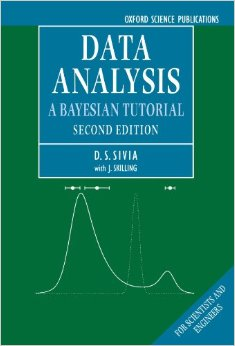
\includegraphics[keepaspectratio,width=\textwidth,height=150pt]{figures/sivia.jpg}
\end{column}
\begin{column}{0.33\textwidth}
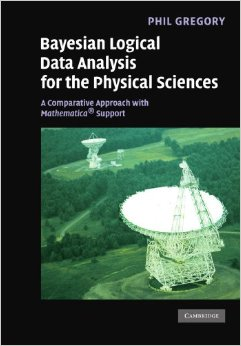
\includegraphics[keepaspectratio,width=\textwidth,height=150pt]{figures/gregory.jpg}
\end{column}
\begin{column}{0.33\textwidth}
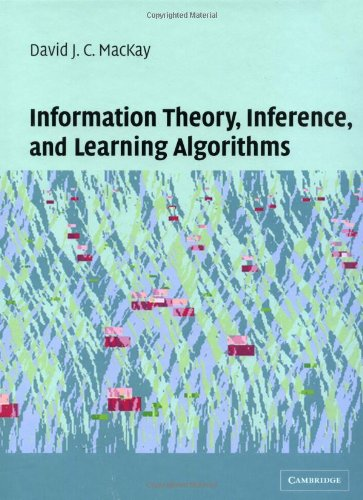
\includegraphics[keepaspectratio,width=\textwidth,height=150pt]{figures/mackay.jpg}
\end{column}
\end{columns}

\end{frame}

\begin{frame}

\frametitle{History}
\label{history}

\begin{itemize}
\item Bernoulli (1713) wondered how the mechanics of deductive logic applied to games of chance
could be applied to inductive logic problems

\item Bayes (1763 - postumous) provided an answer (Bayes' formula) to Bernoulli's questions

\item Laplace (1812) independently derived Bayes' theorem in the more common form we know today

\end{itemize}

Probabilities represent a \emph{plausibility} or \emph{degree-of-beilef} of a proposition given the evidence at hand.

\end{frame}

\begin{frame}

\frametitle{History}
\label{history}

``Probability theory is nothing but common sense reduced to calculation'' - Laplace

\begin{figure}[htbp]
\centering
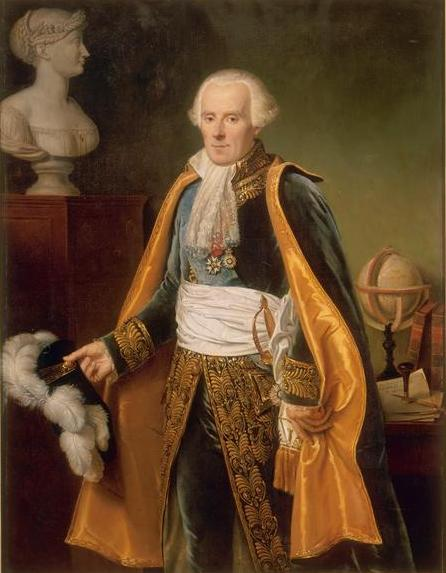
\includegraphics[keepaspectratio,width=\textwidth,height=125pt]{figures/laplace.jpg}
\label{laplace}
\end{figure}

\end{frame}

\begin{frame}

\frametitle{Deductive an inductive reasoning}
\label{deductiveaninductivereasoning}

\begin{itemize}
\item Deductive logic

\begin{itemize}
\item A cause (e.g. a theory) can lead to many effects or outcomes (predictions of the theory)

\end{itemize}

\item Inductive logic

\begin{itemize}
\item Observations can be used to \emph{infer} the \emph{plausibility} their of possible causes (e.g.
different theories or models)

\item Also known as \emph{inverse probability} - learning about a model\slash theory from the data\slash observations

\end{itemize}

\end{itemize}

\end{frame}

\begin{frame}

\frametitle{Deductive logic: an example}
\label{deductivelogic:anexample}

We have a set of statements:

\begin{enumerate}[A.]
\item All observed gravitational waves in the southern hemisphere are circularly polarised
\item A gravitational wave is observed to originate in the southern hemisphere
\item A gravitational wave is observed to be circularly polarised
\end{enumerate}

Suppose statement A (our theory) \emph{is} true:

\begin{itemize}
\item if statement B is true, then statement C is also true

\item if statement C is false, then statement B is also false

\end{itemize}

Statement C is a logical consequence of A and B.

\end{frame}

\begin{frame}

\frametitle{Inductive logic: an example}
\label{inductivelogic:anexample}

\begin{enumerate}[A.]
\item All observed gravitational waves from the southern hemisphere are circularly polarised
\item A gravitational wave is observed to originate in the southern hemisphere
\item A gravitational wave is observed to be circularly polarised
\end{enumerate}

What can we say about B \emph{if} A and C are true?

\end{frame}

\begin{frame}

\frametitle{Inductive logic: an example}
\label{inductivelogic:anexample}


\begin{enumerate}[A.]
\item All observed gravitational waves from the southern hemisphere are circularly polarised
\item A gravitational wave is observed to originate in the southern hemisphere
\item A gravitational wave is observed to be circularly polarised
\end{enumerate}


What can we say about B \emph{if} A and C are true?

Note that Statement A doesn't say that all circularly polarised gravitational waves originate in
the southern hemisphere, but we might say that

\begin{itemize}
\item if C is true then B is more {\color{red} plausible}

\end{itemize}

\end{frame}

\begin{frame}

\frametitle{Plausible reasoning}
\label{plausiblereasoning}

In the 1940s and 50s Cox, Polya and Jaynes formalised the mathematics of inductive logic as
{\color{red} plausible reasoning}

\textbf{Probability measures our degree of belief that something is true}

\end{frame}

\begin{frame}

\frametitle{Plausible reasoning}
\label{plausiblereasoning}

Axioms of Cox~\citep{Cox:1946}~\citep{Cox:1961} combined with Boolean algebra, are sufficient to uniquely
specify the theory of probability:

\begin{enumerate}
\item Degree of belief must be a real number between 0 and 1

\item ``\emph{The probability of an inference on given evidence determines the probability of its
contradictory on the same evidence.}''

\item ``\emph{The probability on given evidence that both of two inferences are true is determined by their
separate probabilities, one on the given evidence, the other on this evidence with the additional
assumption that the first inference is true.}''

\end{enumerate}

\end{frame}

\begin{frame}

\frametitle{Plausible reasoning}
\label{plausiblereasoning}

\begin{enumerate}
\item Degree of plausibility must be a real number between 0 and 1

\begin{itemize}
\item $P(X) = 1~\rightarrow$ we are \emph{certain} that $X$ is true

\item $P(X) = 0~\rightarrow$ we are \emph{certain} that $X$ is false

\end{itemize}

\item Belief in a proposition and its negation are related

\begin{itemize}
\item $P(\text{not } A) = f(P(A))$

\end{itemize}

\item Belied in a pair of propositions $x,y$ ($x$ \emph{and} $y$) is related to the belief in the
conditional proposition $x|y$ (``$x$ given $y$ is true'')

\begin{itemize}
\item $P(x,y) = f(P(x|y), P(y))$

\end{itemize}

\end{enumerate}

\end{frame}

\begin{frame}

\frametitle{Plausible reasoning}
\label{plausiblereasoning}

The degree of belief will always depend on available {\color{red} background information} or
assumptions, $I$.

E.g. we write $P(X|I)$ for the probability that $X$ is true given $I$, where the $|$ denotes
conditional probability:

\begin{itemize}
\item our state of knowledge about $X$ is \emph{conditioned} by the background information\slash assumptions $I$

\end{itemize}

Throughout this course we will use the notation that `$P$' represents a probability, whilst `$p$'
represents a probability density function, such that
\[
P(x_1<X<x_2|I) = \int_{x_1}^{x_2} p(x|I) {\rm d}x.
\]

\end{frame}

\begin{frame}

\frametitle{Rules of probability}
\label{rulesofprobability}

The rules for probabilities of propositions are inherited from classical logic and Boolean algebra:

\begin{itemize}
\item \emph{Law of Excluded Middle} $P(A\text{ or not}(A)) = 1$

\item \emph{Law of Non-contradition} $P(A\text{ and not}(A)) = 0$

\begin{itemize}
\item i.e. $P(A) + P(\text{not }A) = 1$ (the \textbf{sum rule})

\end{itemize}

\item \emph{Association}

\begin{itemize}
\item $P(A,[B,C]) = P([A,B],C)$

\item $P(A \text{ or } [B \text{ or }C]) = P([A \text{ or } B] \text{ or }C)$

\end{itemize}

\item \emph{Distribution}

\begin{itemize}
\item $P(A,[B\text{ or }C]) = P(A,B\text{ or }A,C)$

\item $P(A\text{ or }[B,C]) = P([A\text{ or }B],[A\text{ or }C])$

\end{itemize}

\end{itemize}

\end{frame}

\begin{frame}

\frametitle{Rules of probability}
\label{rulesofprobability}

\begin{itemize}
\item \emph{Commutation}

\begin{itemize}
\item $P(A,B) = P(B,A)$

\item $P(A \text{ or } B) = P(B \text{ or } A)$

\end{itemize}

\item \emph{Duality} (De Morgan's Theorem)

\begin{itemize}
\item $P(\text{not }[A,B]) = P(\text{not}(A) \text{ or } \text{not}(B))$

\item $P(\text{not }[A\text{ or }B]) = P(\text{not}(A),\text{not}(B))$

\end{itemize}

\end{itemize}

\end{frame}

\begin{frame}

\frametitle{Rules of probability}
\label{rulesofprobability}

Note that you may see other notation for probabilities expressed with Boolean logic (this list is
not exhaustive)

\begin{itemize}
\item Negation ($A$ is false)

\begin{itemize}
\item $P(\text{not }A)$, or $P(\bar{A})$, or $P(\lnot A)$

\end{itemize}

\item Logical product (both A \emph{and} B are true)

\begin{itemize}
\item $P(A,B)$, or $P(AB)$, or $P(A\text{ and }B)$, or $P(A\land B)$

\end{itemize}

\item Logical sum (at least one of A \emph{or} B is true)

\begin{itemize}
\item $P(A+B)$, or $P(A\text{ or }B)$, or $P(A\lor B)$

\end{itemize}

\end{itemize}

\end{frame}

\begin{frame}

\frametitle{Rules of probability}
\label{rulesofprobability}

From these axioms we can derive:

\begin{itemize}
\item The \textbf{(Extended) Sum Rule}

\begin{itemize}
\item $P(A\text{ or }B) = P(A) + P(B) - P(A\text{ and }B)$

\end{itemize}

\item The \textbf{Product Rule}

\begin{itemize}
\item $P(A\text{ and }B) = P(A)P(B|A) = P(B)P(A|B)$

\end{itemize}

\end{itemize}

These rules apply to probabilities $P$ and also probability density functions (pdfs) $p$.

\end{frame}

\begin{frame}

\frametitle{Rules of probability}
\label{rulesofprobability}

\emph{Simple demonstration of the extended sum rule.}

What is the probability that a card drawn from a standard deck of cards is a spade \emph{or} an ace?

We have $P(\spadesuit) = 13/52 = 1/4$ and $P(\text{ace}) = 4/52 = 1/13$, and $P(\spadesuit\text{ 
and ace}) = 1/(4\times 13) = 1/52$. It is reasonably obvious that for $P(\spadesuit\text{ or ace})$
we want to sum the probabilities for both cases, however they both contain the case where
$P(\spadesuit\text{ and ace})$, so we have to remove one of those instances

\[
P(\spadesuit\text{ or ace}) = \frac{13 + 4 - 1}{52} = \frac{16}{52}
\]

\end{frame}

\begin{frame}

\frametitle{Bayes' theorem}
\label{bayestheorem}

From the product rule comes
\[
    \boxed{P(B|A,I) = \frac{P(A|B,I)P(B|I)}{P(A|I)}}
\]

This is {\color{red} {\bf Bayes' theorem}}.

From now on we will stick to using $P(A,B|I)$ to denoted the
probability of $A$ \emph{and} $B$, where we have also explicitly added the conditioning on background
information $I$.

\end{frame}

\begin{frame}

\frametitle{Bayes' theorem}
\label{bayestheorem}

Bayes theorem can be cast in terms of a \textbf{model} and some observations, or \textbf{data}. It tells us
how to update our degree of belief about our model based on new data.
\[
\redub{P(\text{model}|\text{data},I)}_{\mathclap{\text{Posterior}}} = 
\frac{\redob{P(\text{data}|\text{model},I)}^{\mathclap{\text{Likelihood}}} 
\redob{p(\text{model}|I)}^{\mathclap{\text{Prior}}}}{\redub{P(\text{data}|I)}_{\mathclap{\text{
Evidence } } } }
\]

We can calculate the these terms (e.g. analytically or numerically on a computer). 

\end{frame}

\begin{frame}

\frametitle{Bayes' theorem}
\label{bayestheorem}

\begin{itemize}
\item \textbf{Prior}: what we knew, or our degree of belief, about our model before taking data

\item \textbf{Likelihood}: the influence of the data in updating our degree of belief

\item \textbf{Evidence}: the ``\emph{evidence}'' for the data, or the likelihood for the data \emph{marginalised} over
the model (we'll explore this later, but at the moment note it as a constant normalisation factor
for the posterior)

\item \textbf{Posterior}: our new degree of belief about our model in light of the data

\end{itemize}

\end{frame}

\begin{frame}

\frametitle{Bayes' theorem}
\label{bayestheorem}

A degree of belief was the original way that Bayes and Laplace interpreted probabilities.

But, throughout much of the 20th century the {\color{red} frequentist approach} has dominated.
Reasons included:

\begin{itemize}
\item many saw the idea of probability as a \emph{degree of belief} too subjective

\item too slow\slash difficult to calculate

\end{itemize}

whereas the frequentist approach was

\begin{itemize}
\item \emph{supposedly} objective

\item provided simple ``cookbook'' of procedures to follow

\end{itemize}

\end{frame}

\begin{frame}

\frametitle{Frequentist approach}
\label{frequentistapproach}

Rather than being a \emph{degree of belief} (or plausibility) this approach states

\begin{itemize}
\item Probability = `long run relative frequency' of an event

\end{itemize}

which, \emph{in principle}, could be measured objectively.

\end{frame}

\begin{frame}

\frametitle{Frequentist approach}
\label{frequentistapproach}

If rolling a die what is the probability of rolling a one?

If the die is `fair' we expect $P(1)=P(2)=\ldots=p(6) = 1/6$.

However, imagine we don't know the die is fair. How would we go about finding these
probabilities and seeing if it is?

We can imagine rolling the dice $M$ times, and count the number of each outcome, so we define

\[
P(1) = \lim_{M\rightarrow\infty} \frac{n(1)}{M}\text{, and if }P(1) = 1/6\text{ the die is `fair'}
\]

\end{frame}

\begin{frame}

\frametitle{Frequentist approach}
\label{frequentistapproach}

What do we do to estimate probabilities in the frequentist approach if $M \ne \infty$? I.e. what do
we do if we just have one set of observations?

We will discuss some of the \emph{machinary} to do this later.

\end{frame}

\begin{frame}

\frametitle{Frequentist vs. Bayesian approach}
\label{frequentistvs.bayesianapproach}

\begin{itemize}
\item Frequentist

\begin{itemize}
\item data are a \textbf{repeatable} random sample

\item true parameter \textbf{remain fixed} during this repeatable process

\end{itemize}

\item Bayesian

\begin{itemize}
\item data are an observation from the realised sample

\item parameters are unknown and described probabilistically

\end{itemize}

\end{itemize}

The supposed objectivity of the frequentist approach is illusory. All statistical models, be they
Bayesian or Frequentist, contain assumptions, but it is important to be up front about them.

\begin{center}Subjective $\ne$ arbitrary\end{center}

\end{frame}

\begin{frame}

\frametitle{More rules of probability: marginalisation}
\label{morerulesofprobability:marginalisation}

If we have a set of $M$ discrete propositions $\{x_k:k=1,\ldots,M\}$, conditional on another
proposition $y$, that cover all possibilities, then
\[
\sum_{k=1}^M P(x_k|y,I) = 1
\]

Applying the product rule: $P(x_k,y|I) = P(x_k|y,I)P(y|I)$, we get
\[
\sum_{k=1}^M  P(x_k,y|I) = \underbrace{\left[ \sum_{k=1}^M P(x_k|y,I) \right]}_{=1} P(y|I)
\]

\end{frame}

\begin{frame}

\frametitle{More rules of probability: marginalisation}
\label{morerulesofprobability:marginalisation}

So, the probability of $y$ summed over $x$s, i.e. the marginalised probability for $y$, is
\[
P(y|I) = \sum_{k=1}^M  P(x_k,y|I) 
\]
This extends to the continuum limit in $x$
\[
p(y|I) = \int_{-\infty}^{\infty} p(x,y|I) {\rm d}x
\]
where $p(y|I)$ and $p(x,y|I)$ are \emph{probability density functions} (pdfs).

\end{frame}

\begin{frame}

\frametitle{More rules of probability: marginalisation}
\label{morerulesofprobability:marginalisation}

To calculate a probability from a pdf we can find the area under it
\[
P(a\le x \le b|I) = \int_a^b p(x|I) {\rm d}x
\]
where we also have the normalisation condition that
\[
\int_{-\infty}^{\infty} p(x|I) {\rm d}x = 1.
\]

\end{frame}

\begin{frame}

\frametitle{More rules of probability}
\label{morerulesofprobability}

In the Bayesian approach the probabilities defined above can be for any proposition, however in the
frequentist approach probabilities only apply to discussion of \textbf{random variables}.

\begin{itemize}
\item \textbf{Random variable} (RV) is ``a quantity that can meaningfully vary throughout a series of repeated
experiments''

\begin{itemize}
\item E.g. a measured physical quantity (such as height, weight, gravitational wave amplitude) which contains random errors

\end{itemize}

\end{itemize}

The \emph{random variable} therefore could represent data (and as we will discuss in Parts 2 \& 3 could be
conditional on other parameters).

\end{frame}

\begin{frame}

\frametitle{Some important pdfs: discrete case}
\label{someimportantpdfs:discretecase}

Discrete pdfs involve processes where the \emph{random variable} can only be a positive integer.

\textbf{Poisson pdf}: for data involving number counts

\begin{itemize}
\item e.g. number of photons per second counted by a CCD

\end{itemize}

Probability of a certain number of detections, $r$:
\[
\boxed{p(r) = \frac{\mu^r e^{-\mu}}{r!}}
\]

Poisson pdf assumes detections and independent and the rate $\mu$ is constant.

\end{frame}

\begin{frame}

\frametitle{Some important pdfs: discrete pdf}
\label{someimportantpdfs:discretepdf}

\begin{figure}[htbp]
\centering
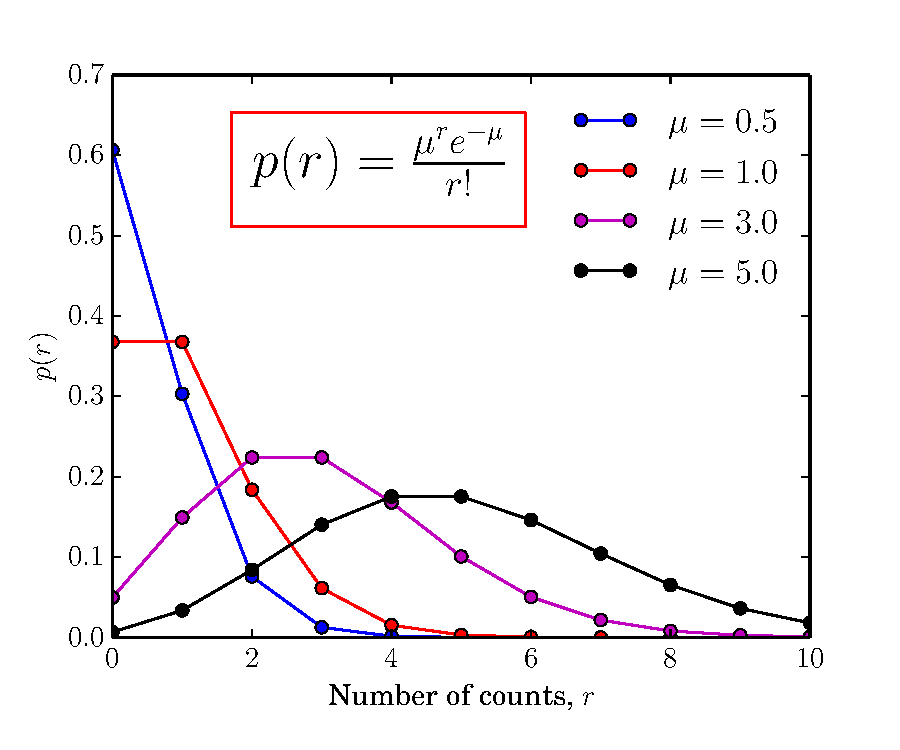
\includegraphics[keepaspectratio,width=\textwidth,height=210pt]{figures/poisson.pdf}
\label{poisson}
\end{figure}

\end{frame}

\begin{frame}

\frametitle{Some important pdfs: Binomial pdf}
\label{someimportantpdfs:binomialpdf}

\textbf{Binomial pdf}: number of successes from $N$ observations for two mutually exclusive outcomes
(i.e. `heads' or `tails' from a coin toss)

Probability of a certain number of successes, $r$:
\[
\boxed{p_N(r) = \frac{N!}{r!(N-r)!}\theta^r(1-\theta)^{N-r}}
\]

where $\theta$ is the probability of `success' for a single outcome, e.g. the coin comes up heads
(which for a fair coin means $\theta = 0.5$).

\end{frame}

\begin{frame}

\frametitle{Some important pdfs: Binomial pdf}
\label{someimportantpdfs:binomialpdf}

\begin{figure}[htbp]
\centering
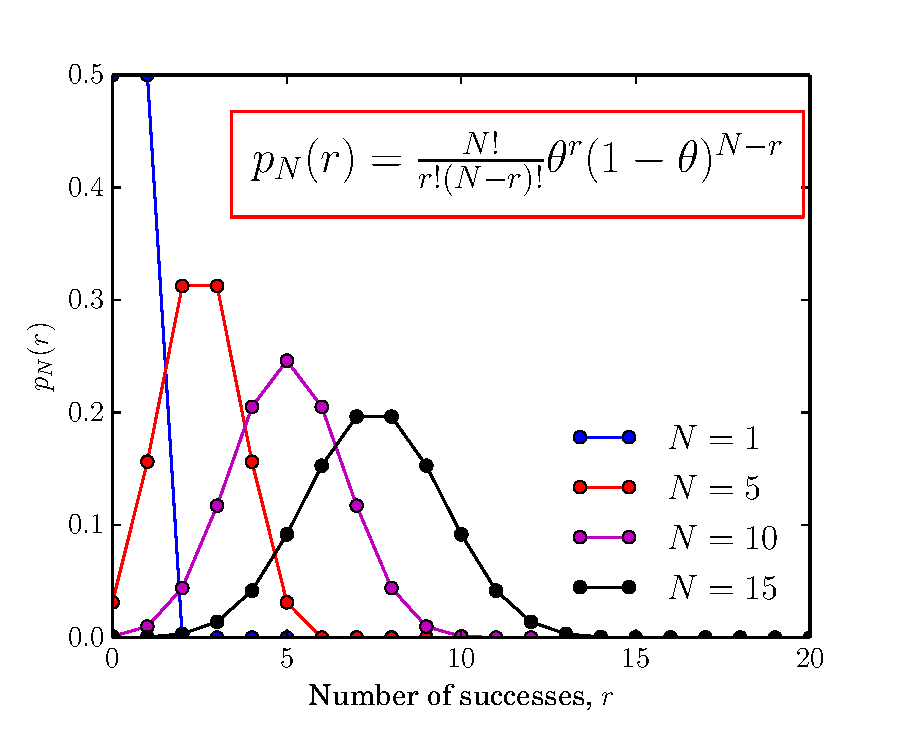
\includegraphics[keepaspectratio,width=\textwidth,height=210pt]{figures/binomial.pdf}
\label{binomial}
\end{figure}

\end{frame}

\begin{frame}

\frametitle{Some important pdfs: discrete case}
\label{someimportantpdfs:discretecase}

In the discrete cases
\[
\sum_{r=0}^{\infty} p(r) = 1,
\]
so $p$ is the probability of a given outcome.

E.g. for the binomial case, given $\theta = 0.5$ as the chance of getting a head in a single coin
toss is, the probability $p_{N=1}(r=1) = 0.5$.

\end{frame}

\begin{frame}

\frametitle{Some important pdfs: Continuous case}
\label{someimportantpdfs:continuouscase}

Continuous pdfs are used when a \emph{random variable} can be defined over a continuum of possible real
values.

\textbf{Uniform pdf}: probability is uniform within a range and zero elsewhere
\[
p(x) =
  \begin{cases}
    \frac{1}{b-a},& \text{if } a < x < b \\
    0,              & \text{otherwise}
  \end{cases}
\]

\end{frame}

\begin{frame}

\frametitle{Some important pdfs: Continuous case}
\label{someimportantpdfs:continuouscase}

\textbf{Central, Normal, or Gaussian pdf}: probability has a bell-shaped distribution about a mean value
$\mu$, with a width $\sigma$ (the standard deviation)
\[
\boxed{p(x) = \frac{1}{\sqrt{2\pi\sigma^2}}\exp{\left[-\frac{1}{2\sigma^2}(x-\mu)^2 \right]} \equiv N(\mu,\sigma^2)}
\]

\end{frame}

\begin{frame}

\frametitle{Some important pdfs: Continuous case}
\label{someimportantpdfs:continuouscase}

\begin{figure}[htbp]
\centering
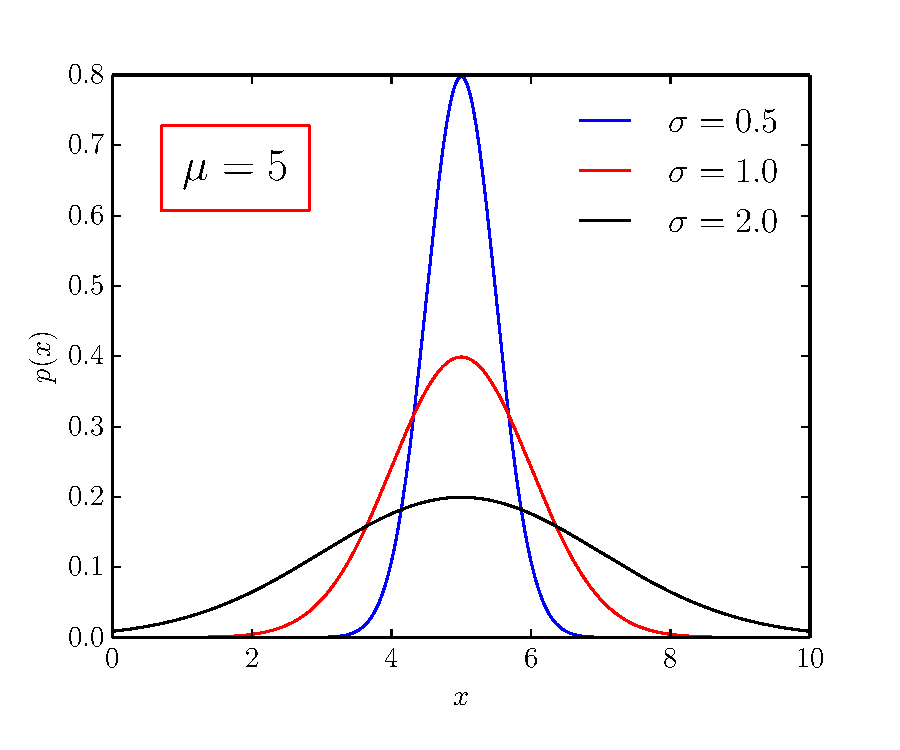
\includegraphics[keepaspectratio,width=\textwidth,height=210pt]{figures/gaussian.pdf}
\label{gaussian}
\end{figure}

\end{frame}

\begin{frame}

\frametitle{Cumulative distribution function (CDF)}
\label{cumulativedistributionfunctioncdf}

Given a pdf, $p(x)$, the CDF defines the intergrated probability up to a given value $z$.
\[
\boxed{P(z) = \int_{-\infty}^{z} p(x) {\rm d}x = \text{Prob}(x<z)}
\]

Note that the pdf is therefore the derivative of the CDF.

\end{frame}

\begin{frame}

\frametitle{Cumulative distribution function (CDF)}
\label{cumulativedistributionfunctioncdf}

\begin{figure}[htbp]
\centering
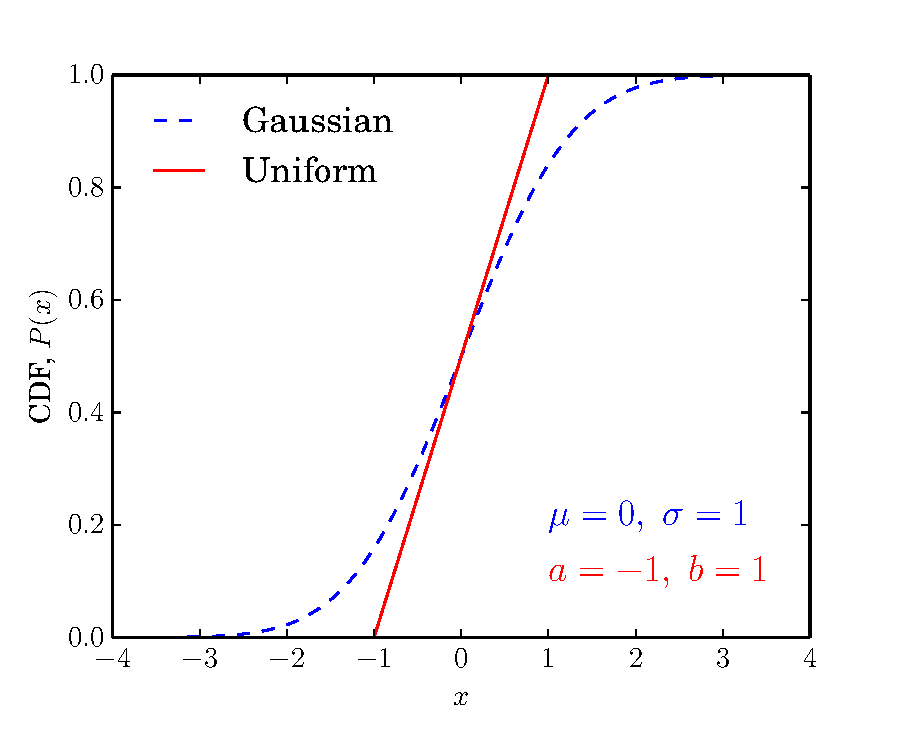
\includegraphics[keepaspectratio,width=\textwidth,height=210pt]{figures/cdfs.pdf}
\label{cdf}
\end{figure}

\end{frame}

\begin{frame}

\frametitle{Moments of a pdf}
\label{momentsofapdf}

The $n^{\rm th}$ \textbf{moment} of a pdf is defined as:
\[
\langle x^n \rangle = 
\begin{cases}
    \sum_{x=0}^{\infty} x^n p(x|I) & \text{\color{red} Discrete case}\\
    \int_{-\infty}^{\infty} x^n p(x|I) {\rm d}x & \text{\color{red} Continuous case}
\end{cases}
\]
The $n^{\rm th}$ \textbf{central moment}, where the origin is the mean, is defined by
\[
\langle (x-\mu)^n \rangle = 
\begin{cases}
    \sum_{x=0}^{\infty} (x-\mu)^n p(x|I) & \text{\color{red} Discrete case}\\
    \int_{-\infty}^{\infty} (x-\mu)^n p(x|I) {\rm d}x & \text{\color{red} Continuous case}
\end{cases}
\]

\end{frame}

\begin{frame}

\frametitle{Moments of a pdf}
\label{momentsofapdf}

The $1^{\rm st}$ moment is called the \textbf{expectation value} (or commonly the \textbf{mean})
\[
E(x) = \langle x \rangle = 
\begin{cases}
    \sum_{x=0}^{\infty} x p(x|I) & \text{\color{red} Discrete case}\\
    \int_{-\infty}^{\infty} x p(x|I) {\rm d}x & \text{\color{red} Continuous case}
\end{cases}
\]
The $2^{\rm nd}$ moment is called the \textbf{mean square}:
\[
\langle x^2 \rangle = 
\begin{cases}
    \sum_{x=0}^{\infty} x^2 p(x|I) & \text{\color{red} Discrete case}\\
    \int_{-\infty}^{\infty} x^2 p(x|I) {\rm d}x & \text{\color{red} Continuous case}
\end{cases}
\]

\end{frame}

\begin{frame}

\frametitle{Moments of a pdf}
\label{momentsofapdf}

The \textbf{variance} (second \emph{central} moment) is defined as:
\[
\text{var}[x] = \sigma^2 = \langle (x-\mu)^2 \rangle = 
\begin{cases}
    \sum_{x=0}^{\infty} (x-\langle x \rangle)^2 p(x|I) & \text{\color{red} Discrete case}\\
    \int_{-\infty}^{\infty} (x-\langle x \rangle)^2 p(x|I) {\rm d}x & \text{\color{red} Continuous 
case}
\end{cases}
\]
where $\sigma$ is called the \textbf{standard deviation}.

In general the variance is given by:
\[
\boxed{\text{var}[x] = \langle x^2 \rangle - \langle x \rangle^2}
\]
The next two \emph{central} moments are called \textbf{skewness} and \textbf{kurtosis}, which for a normal distribution
measure the ``lopsidedness'' and width of the distribution's tails respectively.

\end{frame}

\begin{frame}

\frametitle{Moments and measures of a pdf: example}
\label{momentsandmeasuresofapdf:example}

The mean ($\langle x \rangle = \sum_{x=0}^{\infty} xp(x)$) of the Poisson pdf:
\begin{align*}
    \langle x \rangle &= \sum_{x=0}^{\infty} x\frac{\mu^x e^{-\mu}}{x!} \\
    &= e^{-\mu}\sum_{x=0}^{\infty} x\frac{\mu^x }{x!} \\
    &= e^{-\mu}\mu\redub{\sum_{x=1}^{\infty}\frac{\mu^{x-1}}{(x-1)!}}_{\mathclap{=e^\mu~\text{via}~
    e^y = \sum_{n=0}^{\infty}\frac{y^n}{n!}}} = \mu,
\end{align*}

\end{frame}

\begin{frame}

\frametitle{Moments and measures of a pdf}
\label{momentsandmeasuresofapdf}

\begin{table}[htbp]
\begin{minipage}{\linewidth}
\setlength{\tymax}{0.5\linewidth}
\centering
\small
\begin{tabulary}{\textwidth}{@{}LLLL@{}} \toprule
&$p(x)$&mean ($\langle x \rangle$)&variance\\
\midrule
Poisson&$\frac{\mu^x e^{-\mu}}{x!}$&$\mu$&$\mu$\\
Binomial&$\frac{N!}{x!(N-x)!}\theta^x(1-\theta)^{N-x}$&$N\theta$&$N\theta(1-\theta)$\\
Uniform&$\frac{1}{b-a}$&$\frac{1}{2}(a+b)$&$\frac{1}{12}(b-a)^2$\\
Normal&$\frac{1}{\sqrt{2\pi\sigma^2}}\exp{\left[\frac{(x-\mu)^2}{2\sigma^2}\right]}$&$\mu$&$\sigma^2$\\

\bottomrule

\end{tabulary}
\end{minipage}
\end{table}

\end{frame}

\begin{frame}

\frametitle{Moments and measures of a pdf}
\label{momentsandmeasuresofapdf}

The \textbf{median} value divides the CDF into two equal halfs:
\[
P(x_{\rm median}) = \int_{-\infty}^{x_{\rm median}} p(x) {\rm d}x = 0.5.
\]
The \textbf{mode} is the value of $x$ for which the pdf is a \textbf{maximum} (modes of pdfs may not be
uniquely defined, i.e. they can have more than one mode), i.e.
\[
\frac{\partial p(x=x_{\rm mode})}{\partial x} = 0
\]
For a normal pdf we have $\text{mean} = \text{median} = \text{mode} = \mu$.

\end{frame}

\begin{frame}

\frametitle{Variance of a function}
\label{varianceofafunction}

The variance of an arbitrary function of some random variable $x$ can be approximated by
\[
\boxed{\text{var}[f(x)] = \text{var}[x]\left(\frac{\partial f}{\partial x}\right)^2_{x=\bar{x}}}
\]
where $\bar{x}$ is the mean of $x$. E.g. we measure variable $x$, but we want to determine the
variance of $f(x) = y = x^2$, then we have
\[
\text{var}[f(x)] = 4\sigma^2_x \bar{x}^2. 
\]

\end{frame}

\begin{frame}

\frametitle{Change of variables in pdf}
\label{changeofvariablesinpdf}

If the pdf of the variable $x$ is $p(x|I)$ and we have some function of $x$, $y=f(x)$ then what is the
pdf, $p(y|I)$, of that function?

We require that probabilities over equivalent intervals are equal, so provided there is a one-to-one
mapping between $x$ and $y$ we have
\[
\int_{x_1}^{x_2} p(x|I) {\rm d}x = \int_{y_1=f(x_1)}^{y_2=f(x_2)} p(y|I) {\rm d}y,
\]
and
\[
p(y|I) = \redub{\left|\frac{{\rm d}x}{{\rm d} y}\right|}_{\mathclap{\text{Jacobian}}}p(x|I)
\]

\end{frame}

\begin{frame}

\frametitle{Change of variables in pdf}
\label{changeofvariablesinpdf}

More generally, if there is not a unique mapping between $x$ and $y$ we would have
\[
p(y|I) = \sum_{f(x_i)=y} \left|\frac{{\rm d}x}{{\rm d} y}\right|_{x_i} p(x_i|I)
\]
This can be expended to the multivariate case where $M$ parameters $\{X_i\}$ map to $M$ parameters $\{Y_i\}$ with
\[
p(\{X_i\}|I) = p(\{Y_i\}|I) \times \redub{\left| \frac{\partial (Y_1, Y_2, \ldots, Y_M) }{\partial (X_1, X_2, \ldots, X_M) } \right|}_{\mathclap{\text{Jacobian}}}
\]
If there relation is between functions with different numbers of variables then change of variables may still be
possible using \href{http://en.wikipedia.org/wiki/Probability\_density\_function\#Example:\_Quotient_distribution}{dummy variables}.

\end{frame}

\begin{frame}

\frametitle{Change of variables: example}
\label{changeofvariables:example}

\begin{columns}
\begin{column}{0.3\textwidth}
Suppose we have $y = \sqrt{x}$, then
\[
\frac{{\rm d}y}{{\rm d}x} = \frac{1}{2x^{1/2}},
\]
and
\begin{align*}
p(y|I) &= \left|\frac{{\rm d}y}{{\rm d} x}\right|^{-1} p(x|I) \\
&= 2x^{1/2}p(x|I).
\end{align*}
\end{column}

\begin{column}{0.7\textwidth}

\begin{figure}[htbp]
\centering
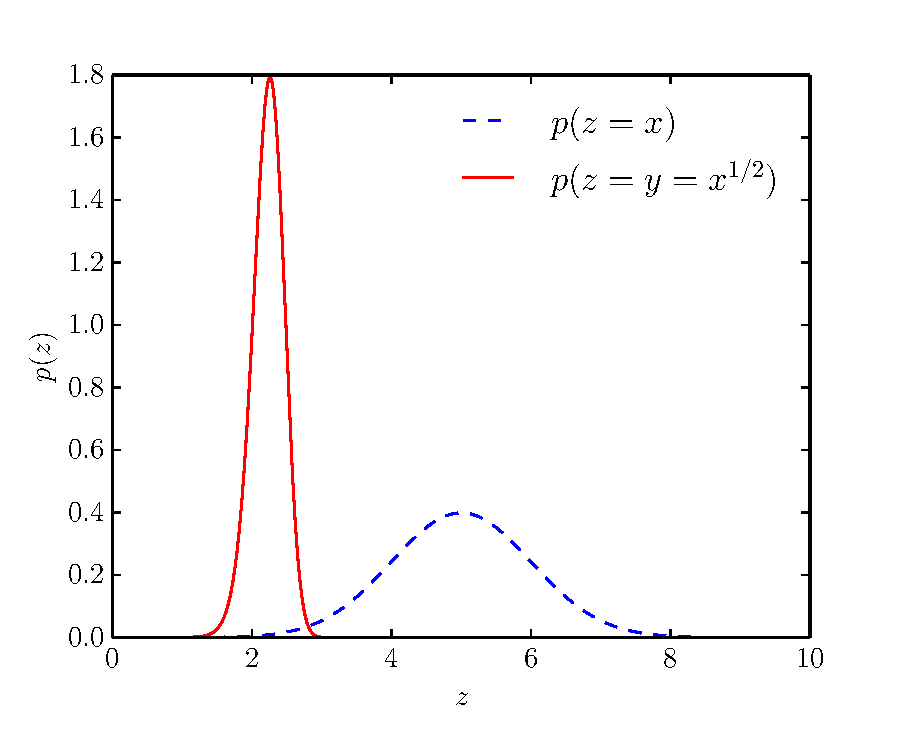
\includegraphics[keepaspectratio,width=\textwidth,height=200pt]{figures/change_of_variables_1d.pdf}
\label{change_of_variables_1d}
\end{figure}

\end{column}
\end{columns}

\end{frame}

\begin{frame}

\frametitle{Multivariate distributions}
\label{multivariatedistributions}

We have so far considered pdfs of single variables (univariate), but we can extend these to the case of
two or more RVs (\textbf{multivariate}).

The \textbf{joint pdf} of two variables $x$ and $y$ is $p(x,y|I)$, where
\[
\text{Prob}(a_1 < x < b_1~\text{and}~a_2 < y < b_2) = \int_{a_1}^{b_1}\int_{a_2}^{b_2} p(x,y|I) {\rm d}x {\rm d}y. 
\]

This extends to any number of variables.

\end{frame}

\begin{frame}

\frametitle{Multivariate distributions: marginal distributions}
\label{multivariatedistributions:marginaldistributions}

Given a \textbf{joint} pdf the marginal pdf on, say, $x$ is given by:
\[
p(x|I) = \int_{-\infty}^{\infty} p(x,y|I) {\rm d}y,
\]
which is a pdf in the sense that

\begin{itemize}
\item $p(x|I) \ge 0$ for all $x$

\item $\text{Prob}(a < x < b) = \int_a^b p(x|I) {\rm d}x$

\item $\int_{-\infty}^{\infty} p(x|I) {\rm d}x = 1$

\end{itemize}

Note that if the allowed range of a variable is known then the integral limits can be over that
range, i.e. equivalent to saying that the probability is zero outside that range.

\end{frame}

\begin{frame}

\frametitle{Multivariate distributions: marginal distributions}
\label{multivariatedistributions:marginaldistributions}

Given any multivariate pdf we can find the marginal pdf on any subset of the variables, e.g.
\[
p(\theta, \phi|I) = \int_{-\infty}^{\infty}\int_{-\infty}^{\infty} p(\theta, \phi, \psi, \lambda|I) {\rm d}\psi {\rm d}\lambda
\]

\end{frame}

\begin{frame}

\frametitle{Multivariate distributions: conditional distributions}
\label{multivariatedistributions:conditionaldistributions}

Suppose we have two variables $x$ and $y$ where $y$ is specified. We can write the \textbf{conditional} pdf
for $x$ \emph{given} the value of $y$ is true as $p(x|y,I)$ (we have already been implicitly using pdfs conditional
on $I$).

From the \textbf{product rule} we can relate the \emph{joint} pdf to the \emph{conditional} pdf via
\[
p(x|y,I) = \frac{p(x,y|I)}{p(y|I)}~\text{and similarly}~p(y|x,I) = \frac{p(x,y|I)}{p(x|I)}.
\]
Re-arranging these two equations leads back to \textbf{Bayes' theorem}
\[
p(x|y,I) = \frac{p(y|x,I)}{p(y|I)}p(x|I)
\]

\end{frame}

\begin{frame}

\frametitle{Multivariate distributions: statistical independence}
\label{multivariatedistributions:statisticalindependence}

If the conditional pdf $p(x|y,I)$ does not depend of $y$ this means that $x$ and $y$ are statistically
independent, i.e. the observed value of $x$ is unaffected by the observed value of $y$.

So, for independent variables we have e.g. $p(x|y,I) = p(x|I)$ and $p(y|x,I) = p(y|I)$, so the joint pdf
can be written
\[
p(x,y|I) = p(x|y,I)p(y|I) = p(x|I)p(y|I)
\]
We can say that a set of variables are \textbf{mutually independent} if their joint pdf can be written as the
product of their marginal pdfs, i.e. $n$ variables $x_n$ are independent if
\[
p(x_1,x_2,\ldots,x_n|I) = p(x_1|I)p(x_2|I)\ldots p(x_n|I).
\]

\end{frame}

\begin{frame}

\frametitle{Multivariate distributions: bivariate normal pdf}
\label{multivariatedistributions:bivariatenormalpdf}

A commonly used joint pdf for two variables $x$ and $y$ is the \textbf{bivariate normal} pdf, which has form
\[
p(x,y|I) = \frac{1}{2\pi\sigma_x\sigma_y\sqrt{1-\rho^2}}\exp{\left[-\frac{1}{2(1-\rho^2)}Q(x,y)\right]}
\]
where $Q(x,y)$ is a quadratic given by
\[
Q(x,y) = \left(\frac{x-\mu_x}{\sigma_x}\right)^2 + \left(\frac{y-\mu_y}{\sigma_y}\right)^2 - 2\rho\left(\frac{x-\mu_x}{\sigma_x}\right)\left(\frac{y-\mu_y}{\sigma_y}\right).
\]
This is defined by the parameters $\mu_x$, $\mu_y$, $\sigma_x$, $\sigma_y$ and $\rho$. [This can be extended to
a \textbf{multivariate normal} pdf.]

\end{frame}

\begin{frame}

\frametitle{Multivariate distributions: bivariate normal pdf}
\label{multivariatedistributions:bivariatenormalpdf}

The first four parameters are given by:
\begin{align*}
    \mu_x &= E[x] \\
    \mu_y &= E[y] \\
    \sigma_x^2 &= \text{var}[x] \\
    \sigma_y^2 &= \text{var}[y]
\end{align*}
whilst the fifth, $\rho$, is known as the \textbf{correlation coefficient} and satisfies
$\rho \sigma_x \sigma_y = E[(x-\mu_x)(y-\mu_y)]$

\begin{itemize}
\item $\rho = 0$ then $x$ and $y$ are independent.

\item $\rho > 0$ gives a positive correlation - $y$ tends to increase as $x$ increases

\item $\rho < 0$ gives a negative correlation - $y$ tends to decrease as $x$ increases

\end{itemize}

\end{frame}

\begin{frame}

\frametitle{Multivariate distributions: bivariate normal pdf}
\label{multivariatedistributions:bivariatenormalpdf}

$E[(x-\mu_x)(y-\mu_y)]$ is known as the \textbf{covariance} of $x$ and $y$ and is often denoted
by $\text{cov}(x,y)$.

Aside: Generally for any two variables with any pdf we define their covariance as
\[
\text{cov}(x,y) = E[(x-E[x])(y-E[y])].
\]
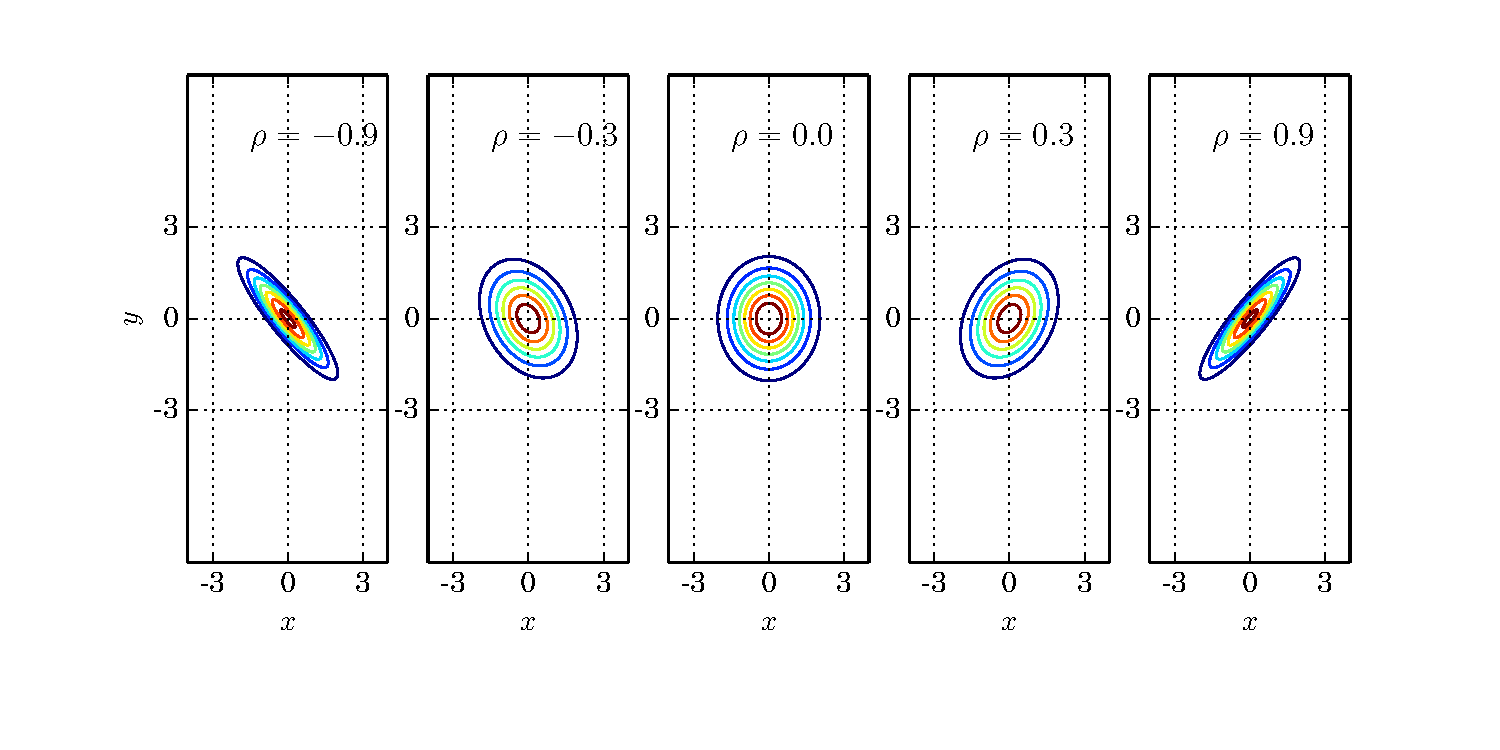
\includegraphics[keepaspectratio,width=\textwidth,height=135pt]{figures/bivariate_normal.pdf}

\end{frame}

\begin{frame}

\frametitle{Multivariate distributions: bivariate normal pdf}
\label{multivariatedistributions:bivariatenormalpdf}

The \textbf{marginal} pdfs of $x$ and $y$ for the bivariate normal pdf are just the univariate
normal pdfs
\begin{align*}
    p(x|I) &= N(\mu_x,\sigma_x^2) \\
    p(y|I) &= N(\mu_y, \sigma_y^2)
\end{align*}

The \textbf{conditional} pdf of $y$ given $x$ is also a univariate normal pdf, but with
\[
p(y|x,I) = N\left(\mu_y + \frac{\sigma_y}{\sigma_x}\rho(x-\mu_x), \sigma_y^2(1-\rho^2)\right),
\]
so as $|\rho| \rightarrow 1$ it can be seen that the width of the conditional distribution tends
to zero.

\end{frame}

\begin{frame}

\frametitle{Multivariate distributions: bivariate normal pdf}
\label{multivariatedistributions:bivariatenormalpdf}

$\mu_y + \frac{\sigma_y}{\sigma_x}\rho(x-\mu_x)$ is often referred to as the \textbf{conditional
expectation} (value) of $y$ given $x$, and the equation
\[
y = \mu_y + \frac{\sigma_y}{\sigma_x}\rho(x-\mu_x)
\]
is called the \textbf{regression line} of $y$ on $x$.

% Bibliography slide 

\end{frame}

\begin{frame}

\frametitle{Bibliography}
\label{bibliography}


\bibliographystyle{unsrt}
\bibliography{stats_part01}


\end{frame}

\mode<all>
\input{mmd-beamer-footer}

\end{document}\mode*

